\chapter{Evaluation}
\label{chapter:Evaluation}

The focus of the evaluation will be on the different runtimes of the various possible backends. These will be evaluated by running varouis prepared Jayvee models on one underlying dataset.

\section{Data source}
\label{section:data_source}

\subsection{Requirements}
%TODO: why not functional vs non-functional
\label{subsection:data_source_requirements}
\begin{enumerate}
	\item The dataset has to be available in a csv format, because the interpreter can only create tables from csv data.
	\item The dataset must contain a column with a numeric data type.
	\item The dataset should be a minimum of $800\text{MB}$, to make the backend's differences in speed visible.
	\item The dataset should not be larger than $3\text{GB}$, because open-datasets are usually not that big. %FIXME: citation needed +  everything.
	\item The dataset must have a licence conformant with the Open Definition. List here: \url{http://opendefinition.org/licenses/} % TODO: explanation.
\end{enumerate}


\subsection{Chosen Dataset}
The chosen dataset is called "Brewery Operations and Market Analysis" and not based on any real wold data, but rather generated by a python script \autocite{dataset}.

\subsubsection{Fulfilled requirements}
- license is \ac{ODbL} so one is fulfilled
- fits within the maximum and minimum filesize
- contains columns with integer and columns with floating point numbers.
- the dataset is contained in a single csv file.

\subsubsection{Biases}
- dataset does not benefit any backend specifically

\section{Parameters}
\label{section:parameters}
- what optimizations to use:
- typescript(none),
- pl: polars tables, columns and block executor, includes transforms but not RustSQLiteLoaderExecutor
- plob: pl + LocalFileToTableInterpreter
- plrs: pl + RustSQLiteLoaderExecutor
- plobrs(plob + plrs)
- how many transformations: none, some, many
- how many lines of data should be processed: $6$ steps $56250$, $112500$, $225000$, $4500000$, $900000$ ,$1800000$
- how often each configuration should be run: 10 times


\section{evaluation tool}
- cli allows to specify one or multiple values for the parameters.
- no value for a parameter means all possible values are used
- create configuration for every possible combination of linecount, transformation amount and activated optimizations (6 * 3 * 5) = 90 configs.
- run each config 10 times, save duration
- calculate average and standard deviation per config

- the output databases are checked for equality using sqldiff

\begin{figure}
	\begin{plantuml}
		@startuml
		start
		while (For each combination of\nlinecount and transform-amount)
		while (For each backend)
		while (10 times)
		:Run config;
		endwhile
		:Calculate average and
		standard deviation;
		endwhile (done)
		:Compare the resulting sqlite
		files using sqldiff;
		endwhile (done)
		stop
		@enduml
	\end{plantuml}
	\caption{The evaluation tool}\label{fig:uml:evalation-tool}
\end{figure}

\subsection{run config}
- the \Verb|head| cli tool prints the first $n$ lines of a file.
- use this to create files with the specified linecount based on \Verb|brewery-data.csv| %FIXME: correct name
\begin{figure}
	\begin{plantuml}
		@startuml
		!pragma useVerticalIf on
		start
		if (no transforms) then (yes)
		if (""plob"" or ""plobrs"" backend) then (yes)
		:""plob-no.jv"";
		stop
		else (""ts"" or ""pl"" ""plrs"" backend)
		:""ts-no.jv"";
		stop
		endif
		elseif (some transforms) then
		if (""plob"" or ""plobrs"" backend) then (yes)
		:""plob-so.jv"";
		stop
		else (""ts"" or ""pl"" ""plrs"" backend)
		:""ts-so.jv"";
		stop
		endif
		else (many transforms)
		if (""plob"" or ""plobrs"" backend) then (yes)
		:""plob-ma.jv"";
		stop
		else (""ts"" or ""pl"" ""plrs"" backend)
		:""ts-ma.jv"";
		stop
		endif
		endif
		@enduml
	\end{plantuml}
	\caption{Picking the correct model}\label{fig:uml:pick-jv-model}
\end{figure}
- if the backend requires the new block, pick one of the models starting with plob, otherwise with ts.
- pick a model with the name fitting trans
- the models get the path of the source file and the path of the destination from a command line parameter (-e)

\begin{listing}
	\begin{minted}{python}
def run_config(interpreter_dir, linecount, transforms, backend):
		source = f"l-{linecount}.csv"
		run f"head --lines=${linecount} brewery_data.csv > {source}" #FIXME: name
		model = ... # See in fig:uml:pick-jv-model
		destination = f"{backend}-{transforms}-{linecount}.sqlite"

		command = f"node dist/apps/interpreter/main.js {model} -e SRC={source} -e SRC {destination}";

		if backend != "ts":
			command += " --use-polars"

		if backend == "plobrs" or backend == "plrs":
			command += " --use-rusqlite"

		start = now()
		execute(command)
		duration =  now() - start
		return duration
	\end{minted}
\end{listing}



\subsection{evaluation models}
- six models exist:
- starting with ts: csv to table is done the usual way, then  *3 for no transforms, some transforms, and many transforms.
- starting with plob: use the new block, then  *3 for no transforms, some transforms, and many transforms.

\subsubsection{no transforms}
\begin{figure}
	\begin{subfigure}[h]{0.4\linewidth}
		\begin{plantuml}
			@startuml
			scale 0.7
				[*] --> LocalFileExtractor
			LocalFileExtractor : filePath: requires SRC
			LocalFileExtractor --> TextFileInterpreter : File
			TextFileInterpreter --> CSVInterpreter : TextFile
			CSVInterpreter : enclosing: '"'
			CSVInterpreter --> TableInterpreter : Sheet
			TableInterpreter: header: true
			TableInterpreter --> SQLiteLoader : Table
			SQLiteLoader: table: "Brewing"
			SQLiteLoader: file: requires DST
			SQLiteLoader --> [*]
			@enduml
		\end{plantuml}
		\caption{ts-no.jv}
	\end{subfigure}
	\hfill
	\begin{subfigure}[h]{0.4\linewidth}
		\begin{plantuml}
			@startuml
			scale 0.7
				[*] --> LocalFileToTableExtractor
			LocalFileToTableExtractor : filePath: requires SRC
			LocalFileToTableExtractor --> SQLiteLoader : Table
			SQLiteLoader: table: "Brewing"
			SQLiteLoader: file: requires DST
			SQLiteLoader --> [*]
			@enduml
		\end{plantuml}
		\caption{plob-no.jv}
	\end{subfigure}
	\caption{Evaluation Pipelines without transforms}
\end{figure}

- no transforms: self explanatory
- some transforms:
- add column with ones
- sum "bitterness + volumes produced" into new col
-  "pH\_level" times 10 000, replace
- square root of total sales, new column


\section{Max file size}
\subsection{ts}

- verified these limits with official jv@0.6.0

\subsubsection{no}
- ts can do 1 900 000 lines (475 mb), can't do 2 000 000 lines(500mb)
- sqlite loader fails with invalid string lenght error when inserting the rows
- sqlite loader might surpass the maximum string length limit when creating the insert values sql statement
\subsubsection{so}
- can't to 1 400 000 lines (350MB) can do 1 300 000 (325MB)
- sqlite loader fails with heap overflow
\subsubsection{ma}
- can't 1 000 000 (250MB) can 900 000 (225MB)
- sqlite loader fails with heap overflow

\subsection{pl}
\subsubsection{no}
- works at 1 800 000 lines (450 mb)
- fails at 1 900 000 lines with heap out of memory, during inserting the rows into the db
- still has typescript implementation of the sqlite loader -> node restrictions apply.
- maybe less memory efficient considering the extracting an loading gets done in typescript

\subsection{plob}
\subsubsection{no}
- works at 1 900 000 lines but not 2 000 000 lines (invalid string lenght error)
- also does sql statement generation in node

\subsection{plrs}
\subsubsection{no}
- can do the 2 000 000 lines the node-sqlite limitations don't apply, it uses the rust stuff
- can't do 2 100 000 lines (525MB) because error: Cannot create a string longer than 0x1fffffe8 (536 870 888) characters.

\subsection{plobrs}
- only plobrs can process the full $10_000_000$ (2.5gb) lines.

%MAYBE TODO: pie chart of supported transfrorms
%TODO: stuff that is not supported by jayvee
\section{the numbers}



\begin{figure}
	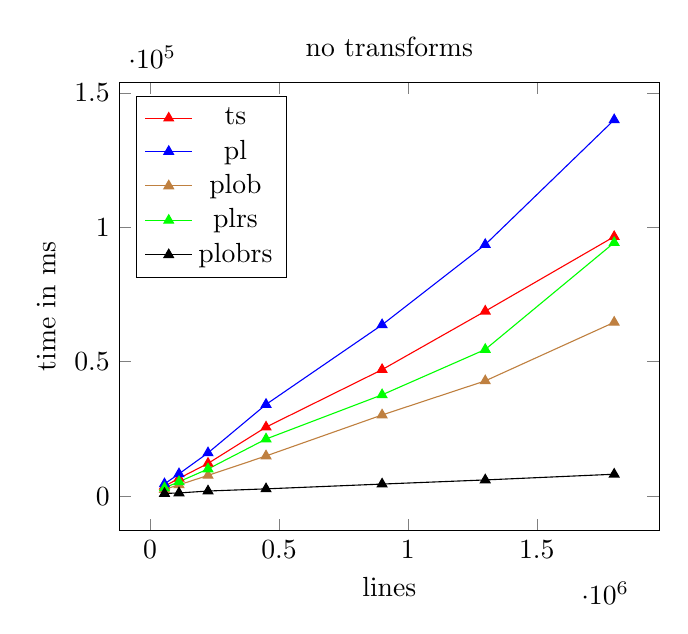
\begin{tikzpicture}
		\begin{axis}[
				title = {no transforms},
				% axis lines = left,
				xlabel = {lines},
				ylabel = {time in ms},
				% xtick={0,56250,112500,225000,450000,900000,1800000},
				legend pos=north west,
			]
			\addplot[
				color = red,
				mark=triangle*,
			]
			coordinates {
					(56250,3724)(112500,6648)(225000,12202)(450000,25701)(900000,47064)(1300000,68801)(1800000,96513)
				};
			\addplot[
				color=blue,
				mark=triangle*,
			]
			coordinates {
					(56250,4581)(112500,8323)(225000,16118)(450000,34125)(900000,63728)(1300000,93559)(1800000,139939)
				};
			\addplot[
				color=brown,
				mark=triangle*,
			]
			coordinates {
					(56250,2531)(112500,4231)(225000,7739)(450000,14976)(900000,30211)(1300000,42888)(1800000,64660)
				};
			\addplot[
				color=green,
				mark=triangle*,
			]
			coordinates {
					(56250,3102)(112500,5390)(225000,10126)(450000,21270)(900000,37705)(1300000,54562)(1800000,94274)
				};
			\addplot[
				mark=triangle*,
			]
			coordinates {
					(56250,1035)(112500,1221)(225000,1936)(450000,2740)(900000,4526)(1300000,6060)(1800000,8184)
				};

			\legend{ts,pl,plob,plrs,plobrs}
		\end{axis}
	\end{tikzpicture}
	\caption{plot no transforms}\label{fig:plot_no_transforms}
\end{figure}

\begin{figure}
	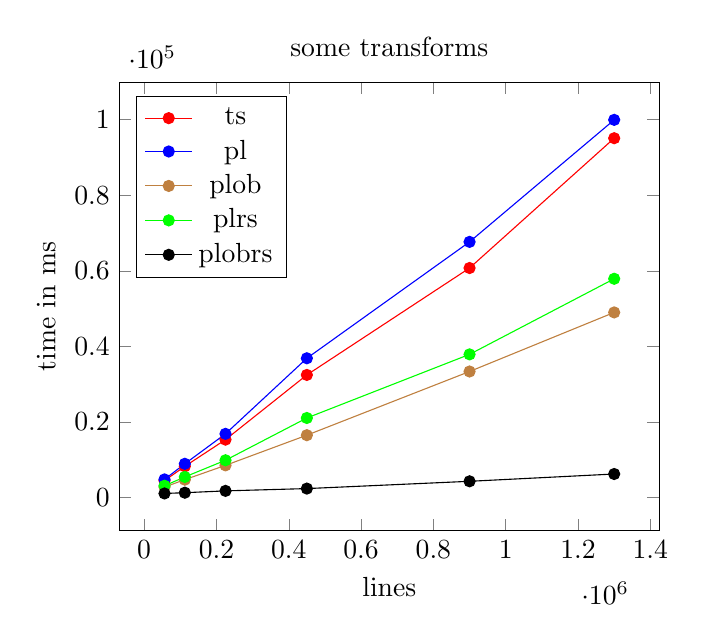
\begin{tikzpicture}
		\begin{axis}[
				title = {some transforms},
				% axis lines = left,
				xlabel = {lines},
				ylabel = {time in ms},
				% xtick={0,56250,112500,225000,450000,900000,1800000},
				legend pos=north west,
			]
			\addplot[
				color = red,
				mark=*,
			]
			coordinates {
					(56250,4495)(112500,8283)(225000,15346)(450000,32467)(900000,60755)(1300000,95102)
				};
			\addplot[
				color=blue,
				mark=*,
			]
			coordinates {
					(56250,4825)(112500,8952)(225000,16881)(450000,36874)(900000,67674)(1300000,99959)
				};
			\addplot[
				color=brown,
				mark=*,
			]
			coordinates {
					(56250,2804)(112500,4756)(225000,8544)(450000,16524)(900000,33375)(1300000,49007)
				};
			\addplot[
				color=green,
				mark=*,
			]
			coordinates {
					(56250,3144)(112500,5479)(225000,9894)(450000,21076)(900000,37910)(1300000,57910)
				};
			\addplot[
				mark=*,
			]
			coordinates {
					(56250,1106)(112500,1305)(225000,1789)(450000,2396)(900000,4323)(1300000,6252)
				};

			\legend{ts,pl,plob,plrs,plobrs}
		\end{axis}
	\end{tikzpicture}
	\caption{plot some transforms}\label{fig:plot_so_transforms}
\end{figure}

\begin{figure}
	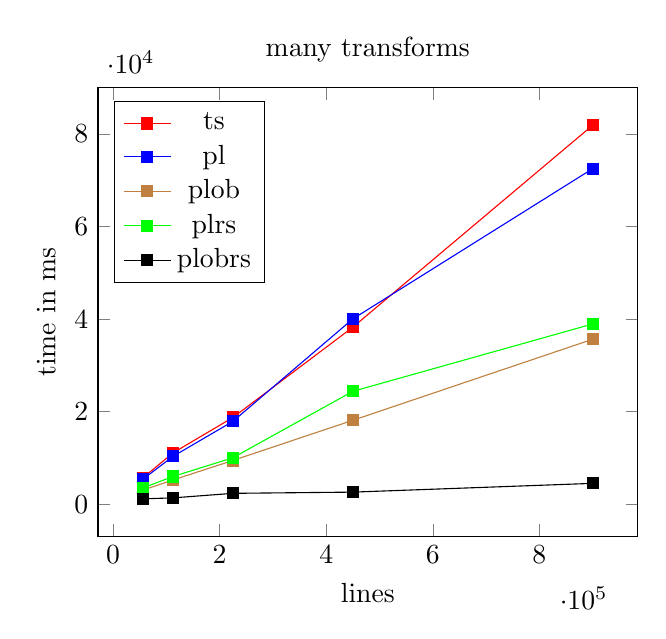
\begin{tikzpicture}
		\begin{axis}[
				title = {many transforms},
				% axis lines = left,
				xlabel = {lines},
				ylabel = {time in ms},
				% xtick={0,56250,112500,225000,450000,900000,1800000},
				legend pos=north west,
			]
			\addplot[
				color = red,
				mark=square*,
			]
			coordinates {
					(56250,5722)(112500,11097)(225000,18750)(450000,38264)(900000,81900)
				};
			\addplot[
				color=blue,
				mark=square*,
			]
			coordinates {

					(56250,5421)(112500,10348)(225000,17914)(450000,40054)(900000,72515)

				};
			\addplot[
				color=brown,
				mark=square*,
			]
			coordinates {

					(56250,3064)(112500,5248)(225000,9470)(450000,18147)(900000,35656)

				};
			\addplot[
				color=green,
				mark=square*,
			]
			coordinates {
					(56250,3545)(112500,5997)(225000,10051)(450000,24406)(900000,38963)
				};
			\addplot[
				mark=square*,
			]
			coordinates {
					(56250,1178)(112500,1383)(225000,2365)(450000,2627)(900000,4518)
				};

			\legend{ts,pl,plob,plrs,plobrs}
		\end{axis}
	\end{tikzpicture}
	\caption{plot many transforms}\label{fig:plot_ma_transforms}
\end{figure}

\begin{figure}
	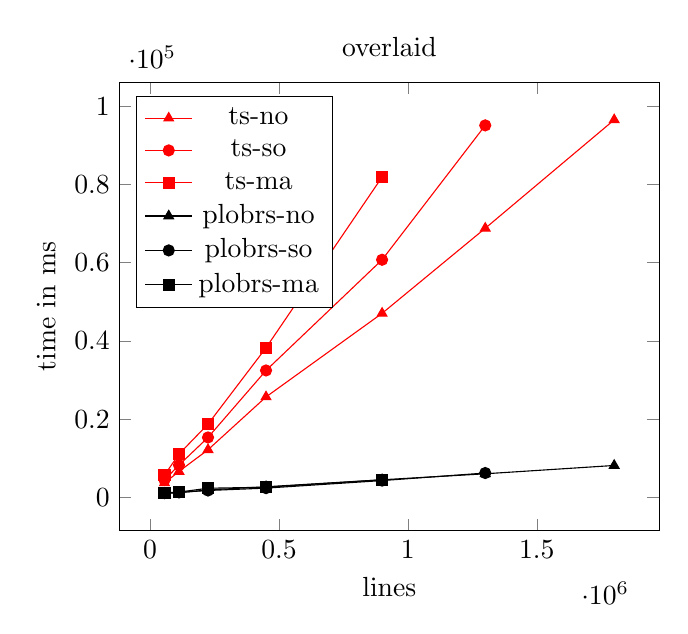
\begin{tikzpicture}
		\begin{axis}[
				title = {overlaid},
				% axis lines = left,
				xlabel = {lines},
				ylabel = {time in ms},
				% xtick={0,56250,112500,225000,450000,900000,1800000},
				legend pos=north west,
			]
			\addplot[
				color = red,
				mark=triangle*,
			]
			coordinates {
					(56250,3724)(112500,6648)(225000,12202)(450000,25701)(900000,47064)(1300000,68801)(1800000,96513)
				};
			\addlegendentry{ts-no}
			\addplot[
				color = red,
				mark=*,
			]
			coordinates {
					(56250,4495)(112500,8283)(225000,15346)(450000,32467)(900000,60755)(1300000,95102)
				};
			\addlegendentry{ts-so}
			\addplot[
				color = red,
				mark=square*,
			]
			coordinates {
					(56250,5722)(112500,11097)(225000,18750)(450000,38264)(900000,81900)
				};
			\addlegendentry{ts-ma}
			\addplot[
				mark=triangle*,
			]
			coordinates {
					(56250,1035)(112500,1221)(225000,1936)(450000,2740)(900000,4526)(1300000,6060)(1800000,8184)
				};
			\addlegendentry{plobrs-no}
			\addplot[
				mark=*,
			]
			coordinates {
					(56250,1106)(112500,1305)(225000,1789)(450000,2396)(900000,4323)(1300000,6252)
				};
			\addlegendentry{plobrs-so}
			\addplot[
				mark=square*,
			]
			coordinates {
					(56250,1178)(112500,1383)(225000,2365)(450000,2627)(900000,4518)
				};
			\addlegendentry{plobrs-ma}
		\end{axis}
	\end{tikzpicture}
	\caption{plot transforms}\label{fig:plot:ts_vs_plobrs}
\end{figure}

\begin{figure}
	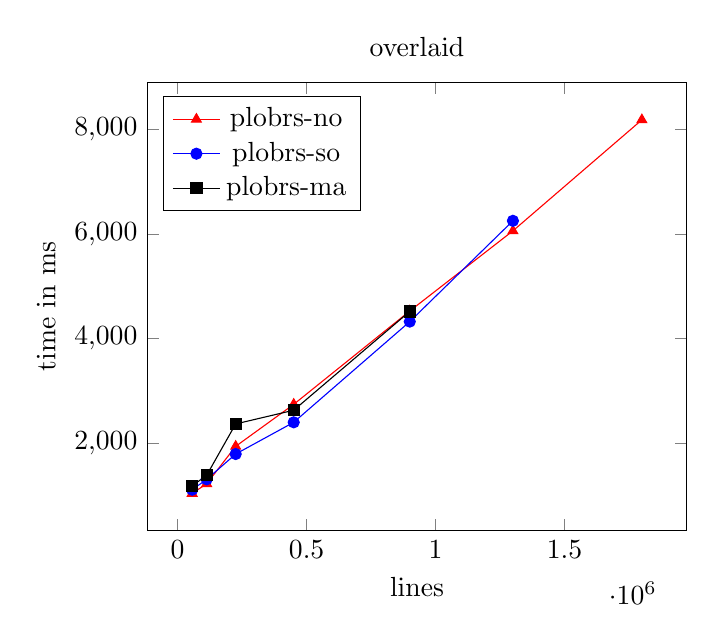
\begin{tikzpicture}
		\begin{axis}[
				title = {overlaid},
				% axis lines = left,
				xlabel = {lines},
				ylabel = {time in ms},
				% xtick={0,56250,112500,225000,450000,900000,1800000},
				legend pos=north west,
			]
			\addplot[
				color = red,
				mark=triangle*,
			]
			coordinates {
					(56250,1035)(112500,1221)(225000,1936)(450000,2740)(900000,4526)(1300000,6060)(1800000,8184)
				};
			\addlegendentry{plobrs-no}
			\addplot[
				color = blue,
				mark=*,
			]
			coordinates {
					(56250,1106)(112500,1305)(225000,1789)(450000,2396)(900000,4323)(1300000,6252)
				};
			\addlegendentry{plobrs-so}
			\addplot[
				mark=square*,
			]
			coordinates {
					(56250,1178)(112500,1383)(225000,2365)(450000,2627)(900000,4518)
				};
			\addlegendentry{plobrs-ma}
		\end{axis}
	\end{tikzpicture}
	\caption{plot transforms}\label{fig:plot:plobrs}
\end{figure}



\subsection{no transforms vs some transforms vs many transforms}
\subsubsection{no transforms}
- pl is slowest, because:
- no transforms yet, so no speedup from there
- from comparing the debug output of two example runs we can see that PolarsSQLiteLoaderExecutor is slower than TsSQLiteLoaderExecutor %TODO: provide numbers
- the one block optimization yields better results than the rust sqlite loader implementation
- plobrs is the best

\subsubsection{some transforms}
- ts is still better than pl but it' close now
- same the introduction of transforms made it closer
- prediction: many transforms will make pl faster
- other than that the same result

\subsubsection{many transforms}
- trend continues, now pl is faster, except once
- the rest remains the same

- TODO: adding transforms increased the runtime by a factor of x

\subsection{ts vs plobrs}
- calculate ts \/ plobrs
- see table
- the more lines, the bigger the ingrease for plobrs,
- the more transforms, the bigger the advantage for plobrs

\begin{figure}
	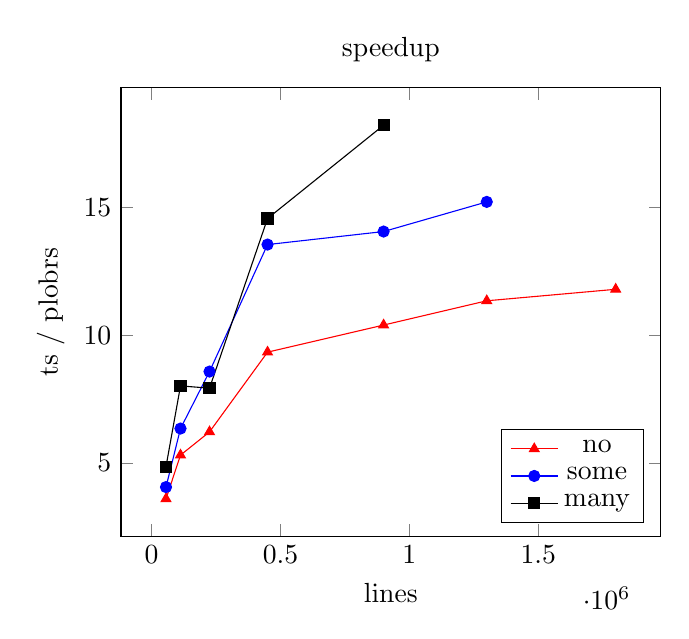
\begin{tikzpicture}
		\begin{axis}[
				title = {speedup},
				% axis lines = left,
				xlabel = {lines},
				ylabel = {ts / plobrs},
				legend pos=south east,
			]
			\addplot[
				color = red,
				mark=triangle*,
			]
			coordinates {
					(56250,3.60)(112500,5.31)(225000,6.22)(450000,9.34)(900000,10.40)(1300000,11.35)(1800000,11.80)
				};
			\addlegendentry{no}
			\addplot[
				color = blue,
				mark=*,
			]
			coordinates {
					(56250,4.06)(112500,6.35)(225000,8.58)(450000,13.55)(900000,14.06)(1300000,15.22)
				};
			\addlegendentry{some}
			\addplot[
				mark=square*,
			]
			coordinates {
					(56250,4.86)(112500,8.02)(225000,7.93)(450000,14.57)(900000,18.22)
				};
			\addlegendentry{many}
		\end{axis}
	\end{tikzpicture}
	\caption{speedup factors}\label{fig:plot:factor}
\end{figure}








\section{Reevaluating the requirements}
\subsection{FR}
1. DONE Polars is columnar, in memory
2. DONE Basic ETL works, otherwise the evaluation wouldn't be possible
3. DONE We used pl.Expr to do this
4. DONE we used napi-rs
5. DONE --use-polars --use-rusqlite
\subsection{NFR}
2. DONE see we lifted the current limit for x at no transforms and increased execution speed by y
3. DONE napi-rs allowed us to hide the rust implementation behind a js library
4. DONE even we used the logger class from execution context where possible and printed to the screen where the logger was unavailable (rust library)
5. DONE we used eslint and prettier to enfoce the project's codestyle. for the rust library we used rustfmt and clippy (linter) defaults
